\chapter{Related Work}\label{chap:relatedWork}
% what exists in this topic area
% What are the differences/similarities to the existing literature? Summarize the findings and identify differences to your own study.
As mentioned in the Introduction there exists various systems in this area, so the Intel True View end-to-end technology solution \cite{intel} is able to render a complete 360-degree replay. The technology behind it is roughly explained in a video \cite{intelvideo} as follows: There are about 38 high-definition 5K cameras installed in a stadium processing terabytes of data every minute across 38 different servers. But the cameras generate not just images of two-dimensional pixels, instead they generate massive amount of volumetric data (voxels), pixels with volume, which allows them to capture height, width and depth. This means you do not lose the depth when capturing a moment with the camera and you are able to map the events in three dimensional space. In the figure \ref{fig:intelcameras} you can see how the 38 cameras are distributed in the stadium to capture the events on the pitch from every angle.
\begin{figure}[h]
	\centering
	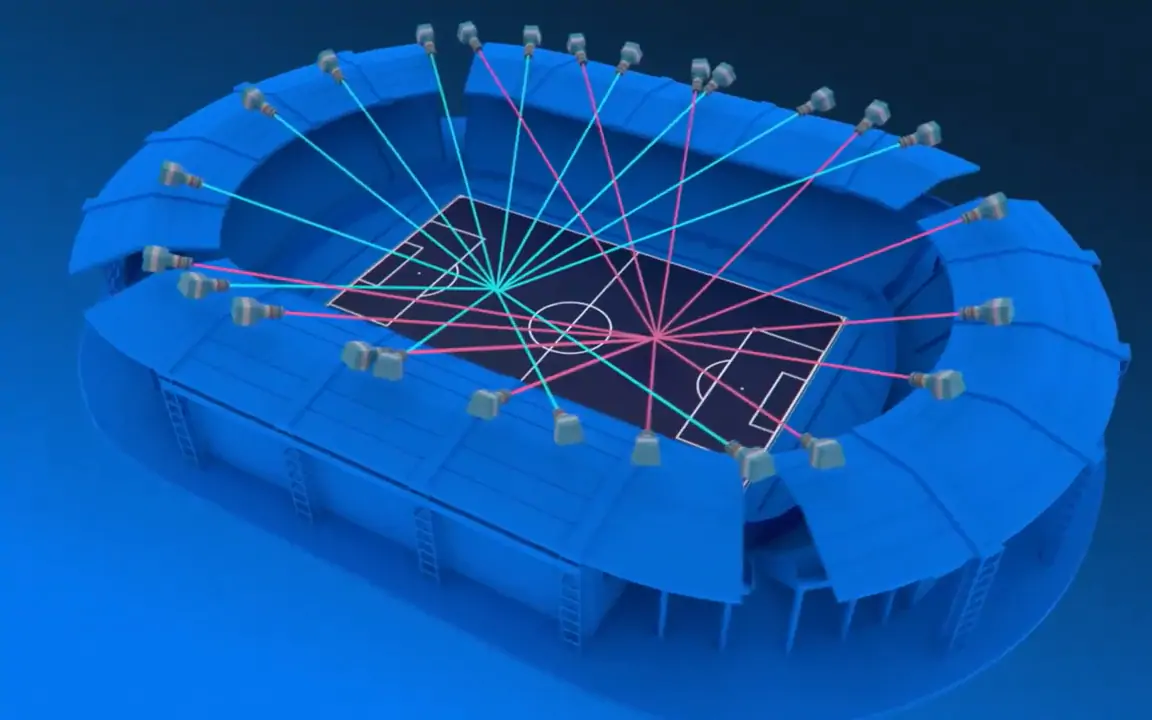
\includegraphics[width=0.7\textwidth]{./images/intelcameras.png}
	\captionsource{High-definiton 5K cameras locations for the Intel True View technology solution in a soccer stadium.\newline}{\cite{intelcameras}}
	\label{fig:intelcameras}
\end{figure}\\
The swiss national soccer team asked to explore state-of-the-art computer vision and visualization technologies for the data of some tv cameras and not to install an expensive system. So what are the possibilities without installing a dozens of high-definition cameras around the stadium to track the bodies of the players. A large related research are has been developed in the last few decades on motion capture technique. 

\section{Motion Capture}
Motion capture tries to track and record the motions of the human body. Whereas the human body is interpreted as a system of rigid links connected by joints as expressed by Xsens \cite{xsens} which is a leading innovator in 3D motion tracking technologies. The developed methods can be divided into different categories, but most technologies do not only benefit from the advantages of one category and combine several techniques to improve the outcome. The main distinction that is particularly relevant for this work is the difference between marker-based motion capture and markerless motion capture \cite{Nogueira2012MotionCF}.

\subsubsection{Marker-Based Motion Capture}
Marker-Based Motion Capture can be further categorized into mechanical, magnetic, acoustic and optical \cite{xsens}. Even the markers are further categorized into active and passive markers. For example passive markers reflect the light back to the cameras in contrast the active markers are equipped with a battery and emit their own light \cite{Nogueira2012MotionCF}.

\begin{itemize}
	\item Mechanical motion system directly track the joints angles using a exoskeleton worn by the person \cite{motionWiki}. This technology is very popular in the film industry. 
	\item Magnetic motion capture systems use the markers as sensors to measure low-frequency magnetic fields generated by a transmitter source. The sensors measure the strength of these magnetic field on order to calculate positions and orientations \cite{magnetic,motionWiki, xsens}. Magnetic systems do not suffer from line of sight problems, thereby the method is useful if the scene is not in the angle of view.
	\item Acoustic tracking systems work with ultrasonic pulses and can compute the position through the time-of-flight of the pulses with triangulation. To work correctly a clear line of sight is needed and to avoid reflections this method should be used outdoors \cite{xsens}.
	\item Optical motion capture uses multiple cameras to track the markers, the markers for this purpose can be passive or active exactly as described above \cite{xsens}. To extract the markers 3D position triangulation is used ad in the acoustic system. There exist even single camera systems but with additionally sensors to measure the lost depth in the image because triangulation is  not possible as noted in \cite{motioncapturetechnologies}.
\end{itemize} 
But in general those approaches are all limited to the fact that the player are required to wear some form of markers on their body. Of course it would be possible to place the markers inside the cloths and shoes but that have to be approved by the FIFA for official games and also by the players themselves. However exactly these technologies are used for video games like the FIFA Football series to capture the movements of the players more realistically.
\begin{figure}[h]
	\centering
	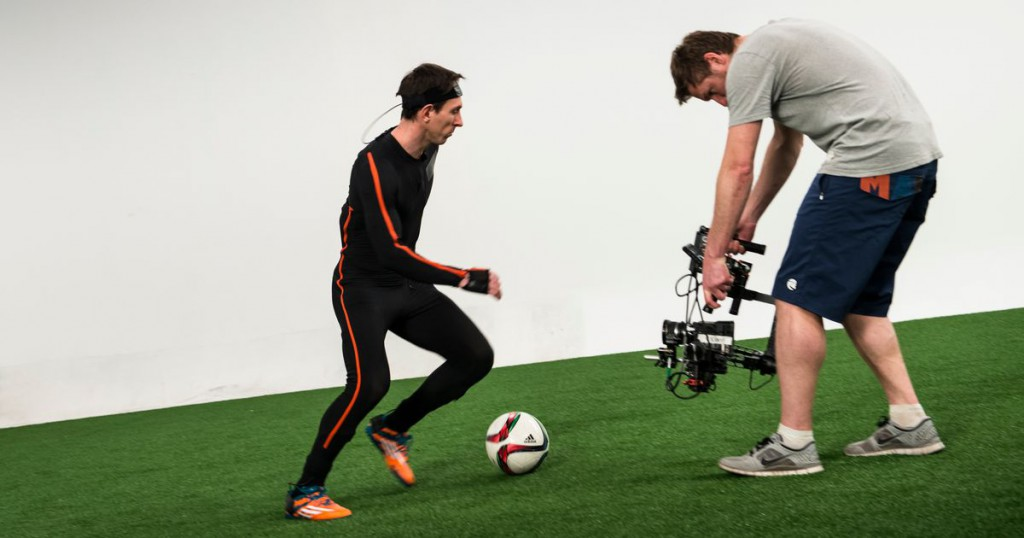
\includegraphics[width=0.7\textwidth]{./images/messi.jpg}
	\captionsource{Messi in Xsens motion capture suit for FIFA 16 to animate his dribbling style as realistically as possible. \newline}{\cite{xsensmessi}}
	\label{fig:messi}
\end{figure}
\subsubsection{Markerless Motion Capture}
Due to the many researches in the field of computer vision, markerless optical motion detection systems are possible. These systems do not rely on a suit with markers which has to be worn, instead they rely on computer vision algorithms to reconstruct the 3D motion from videos and other sensors \cite{motioncapturetechnologies}. 
\begin{figure}[h]
	\centering
	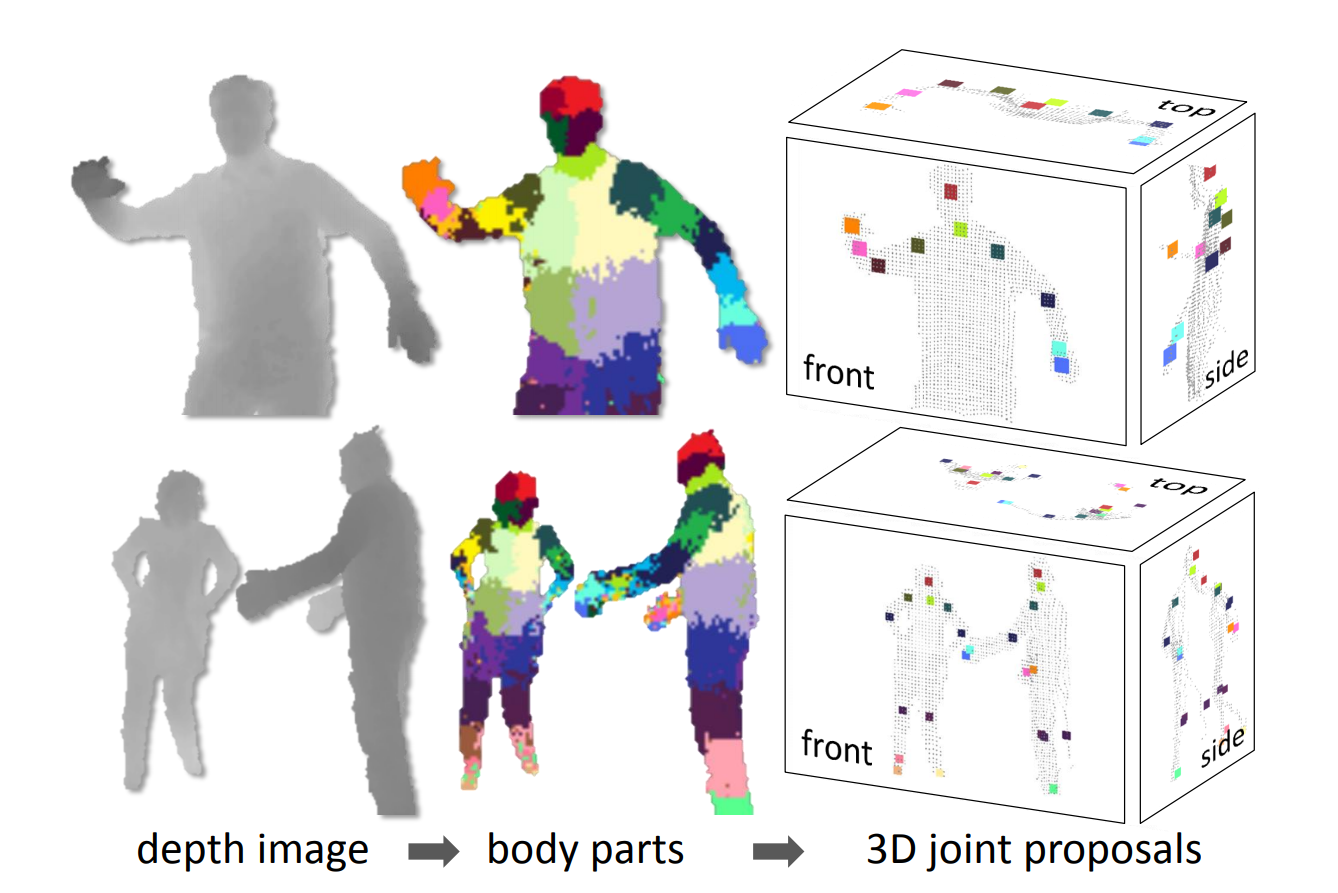
\includegraphics[width=0.7\textwidth]{./images/microsoft.png}
	\captionsource{Overview for the 3D positions reconstruction from one single depth image.\newline}{\cite{microsoft}}
	\label{fig:messi}
\end{figure}
An example for such a system is the Microsoft's Kinect \cite{microsoft}, they localize the 3D positions of body joints from one single depth image. Roughly described they designed an intermediate body parts representation based on an object recognition approach. This presentation consists of several localized body part labels which cover the whole body. This intermediate representation simplifies the difficult pose estimation problem into a simpler classification problem per pixel. But for further reading take a look at the paper \cite{microsoft}.

\section{Human Poses Estimation}
During the last few years the human 2D pose estimation has been greatly improved. Through better object detection algorithms, as the one presented in the section \ref{sec:detectron}, common approaches try to detect a person and run for each detection a single-person pose estimation. The runtime of these so called Top-Down approaches is proportional to the number of detected people in the image \cite{openpose_paper}. To avoid this complexity for multiple people so called buttom-up approaches have been developed as \textit{DeepCut} \cite{deepcut} or \textit{OpenPose} \cite{openpose_paper}. A rough overview how they work is given in the section \ref{sec:openpose} for the \textit{OpenPose} approach. 
\begin{figure}[h]
	\centering
	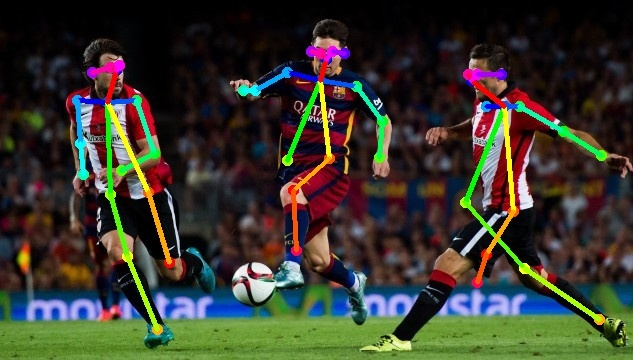
\includegraphics[width=0.7\textwidth]{./images/openpose_example.jpg}
	\captionsource{human 2D pose estimation example with OpenPose\newline}{\cite{openpose_example}}
	\label{fig:openpose_example}
\end{figure}\\
The resulting 2D pose estimation is shown in the figure \ref{fig:openpose_example}. With these technologies we were able to estimate human body joints on two dimensional images which is the beginning for 3D human pose estimations.

In order to understand the 3D geometry the depth is needed but exactly this depth is lost in 2D images. To recover the depth from images or videos there exists already comprehensive work such as \cite{depth_estimation,depth_map}. But these are applied to normal scenes and not explicitly to human bodies. The article \cite{3dpose} describes a method for automatic 3D human pose and shape estimation from a single image. This approach builds upon the 2D joints results of \textit{DeepCut}\cite{deepcut}. Afterwards they fit a statistical body shape model to the 2D joints. The corresponding model is called the \textit{Skinned Multi-Person Linear Model (SMPL)} \cite{smpl} which is a realistic 3D model of the human body learned from thousands of 3D body scans. To fit the model to the 2D joints they minimize an objective function including the error from the projected 3D model joints and the previously estimated 2D joints. In the figure \ref{fig:3dpose_example} an example result from the automatic 3D human pose and shape estimation is presented.
\begin{figure}[h]
	\centering
	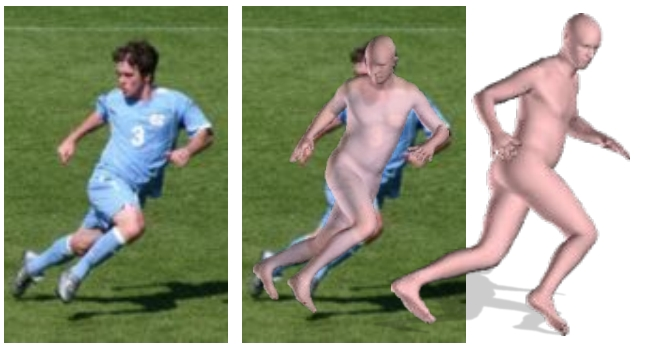
\includegraphics[width=0.7\textwidth]{./images/3dpose_example.jpg}
	\captionsource{To the 2D joints of the original image (not shown) a \textit{SMLP} model is fitted as seen in the middle and on the right side the resulting 3D model is rendered from a different viewpoint. \newline}{\cite{3dpose}}
	\label{fig:3dpose_example}
\end{figure}\\
In contrast to our method they fit a complex statistical body shape model to the 2D joints and end up with a 3D shape model. The three dimensional joint positions are sufficient for our purpose. Additionally we have access to multiple camera views which enables the possibility for triangulation based methods. Along we can benefit from several consecutive frames to not treat each frame individually.


\section{Soccer on Your Tabletop}\label{tabletop}
% general description what they have done
This section presents the main concepts of the project \textit{Soccer on Your Tabletop}\cite{tabletop}. The goal of their work is a moving 3D reconstruction of a soccer game from a single monocular video. The estimation of the depth map of each player represents the core of their work. In the figure \ref{fig:tabletop} a rough overview of their pipeline is given, with the first few steps explained in more detail in the following sections. The reason for the more detailed explanation is their integration in our work which is further outlined in the method chapter.
\begin{figure}[h]
	\centering
	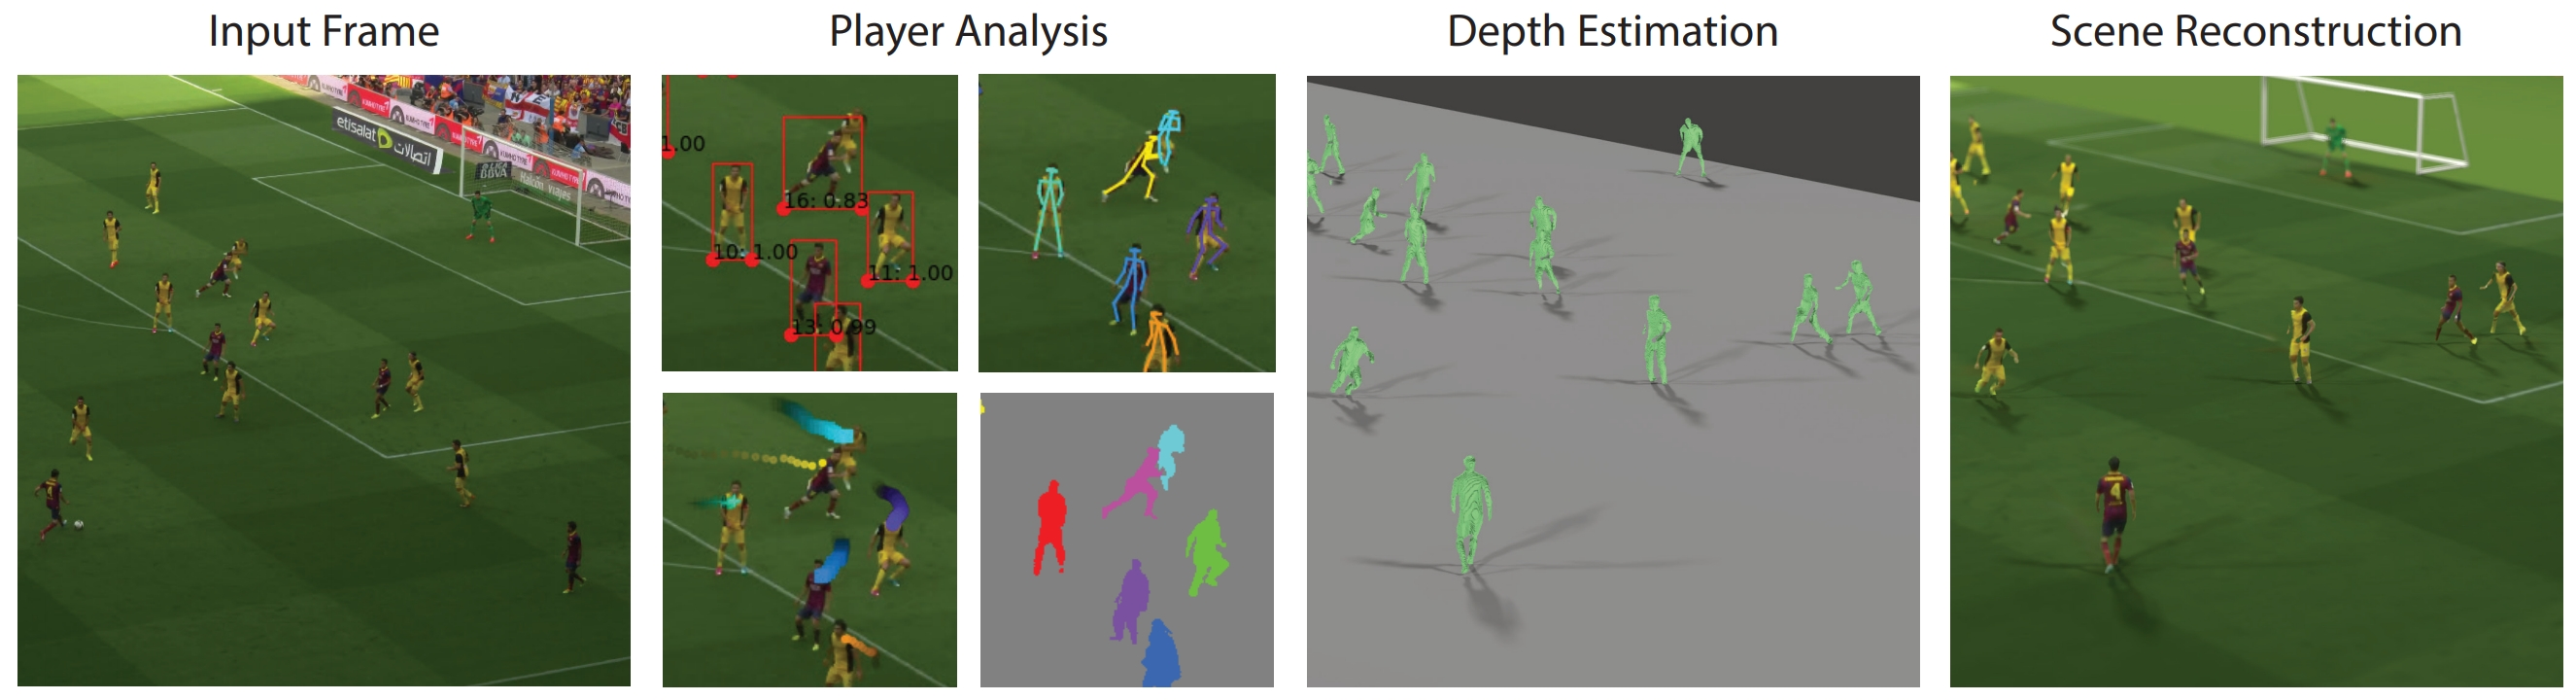
\includegraphics[width=1.\textwidth]{./images/tabletop.jpg}
	\captionsource{Overview of their reconstruction pipeline. In the first step the players from the input frame are analyzed and the camera calibrated. Through the player analysis they segment the player and reconstruct the depth map on the pitch per player. At the end they render the scene in 3D for a complete scene reconstruction. \newline}{\cite{tabletop}}
	\label{fig:tabletop}
\end{figure}

The input are frames from a single monocular video that is being processed. The player analysis consists of several building blocks of existing work. In the first step a state-of-the-art object detection algorithm called \textit{Detectron}\cite{detectron} is used to detect the persons in each frame. The 2D poses for the recognized persons are then determined using \textit{OpenPose}\cite{openpose_paper}. These poses together with the detection are then used to refine the people segmentation \cite{segmentation}. For the per player depth map on the pitch they developed a deep network. The network was trained on video game data, to be more precise they extracted depth maps from EA FIFA games. The advantage of this training data is the specific form in terms of movement, clothing and camera perspective \cite{tabletop}. 

\subsubsection{Building Blocks}
As mentioned above there are multiple building blocks which are also part of our method. For this purpose the theory behind them are further explained in the next few section. How they are integrated into our work is then explained in the method chapter. 


\subsection{Detectron}\label{sec:detectron}
Detectron is a system developed by Facebook AI Research and implements multiple  state-of-the-art object detection algorithms such as Mask R-CNN \cite{r-cnn}, RetinaNet \cite{retinenet} and some others. The system is powered by the Caffe2 deep learning framework which is now part of PyTorch \cite{pytorch}. 

Soccer on your tabletop modified the originally published \textit{infer\_simple.py} file by Detectron which outputs the visualization of the algorithm in PDF format. Instead bounding boxes around the recognized objects and segmentation masks are outputted. At this point in time not only the players but also the spectators and the ball were recognized. In further processing the objects outside of the pitch get removed using the camera calibration and bounding boxes with an area under a specific threshold are removed just to keep the boxes for the players \cite{tabletop}. These are used in later processes. 

\subsection{Calibration}\label{sec:tablecalibration}
During the calibration step, the camera matrix is determined for each frame of a camera. The camera matrix $M$ transforms homogeneous 3D world coordinates to homogeneous 2D image coordinates and can be decomposed into an intrinsic and extrinsic camera matrix. $\mathbf{R}$ and $\mathbf{T}$ build together the extrinsic camera matrix which describes the camera's position and view direction in world coordinates. If you apply the extrinsic matrix to homogeneous 3D world coordinates, they will be transformed by a rotation matrix $\mathbf{R}$ and a translation vector $\mathbf{T}$ to 3D camera coordinates. The intrinsic matrix $\mathbf{A}$ than transforms the 3D camera coordinates to 2D homogeneous screen coordinates. The intrinsic matrix includes the focal length, principal point offsets and the axis skew. The focal length describes the distance between the image plane and the pinhole of the camera. A perpendicular line to the image plane which intersect with the pinhole is called the principal axis. The intersection of the principal axis with the image plane is the principal point and the offsets describe this point with regard to the screen origin. The axis skew is responsible for the shear distortion which is for a true pinhole camera equal to zero \cite{camerablog}.

\subsubsection{Manual Initialization}
The calibration works in two phases, during the first phase four matching pairs of points are selected manually on the first frame and on a 2D reference image of the football field. A matching pair of points consists of the 2D coordinates for the selected point of the first frame and the 3D coordinates for the selected point on the reference image with $z$-coordinates equal to zero. With these point pairs the intrinsic camera matrix $\mathbf{A}$ is determined by a grid search. The grid search estimates for different focal lengths the camera matrices using the \textit{solvePnP} function from the OpenCV library \cite{opencv}. Afterwards the 3D coordinates are projected into the first frame using the previously estimated camera matrices in order to compute a score for the corresponding focal lengths in a least-squares fashion. The result of the grid search are the focal lengths with smallest score and thereby the projection with the smallest error. For the principal point offsets the height and width of the image were simply divided by 2 under the assumption that the principal axis intersects the image at the center. \\
The extrinsic camera matrices are then estimated using the matching pair of points from before with the estimated intrinsic matrix using the \textit{solvePnPRansac} function from the same library. It works in the same fashion as the grid search fo find a solution which minimizes the reprojection error. The use of the \textit{Random sample consensus (RANSAC)}\cite{ransac} scheme, a commonly used iterative method in computer vision which estimates the model parameters using observational data, makes the function robust to outliers \cite{opencv}. 

\subsubsection{Calibration Propagation}
After the manual initialization for the first frame, in the second phase the camera matrices for the next frame are estimated using the matrices from the previous frame. First the edges in the new frame are detected using the canny edge detector \cite{canny}. With the use of the Sobel kernel the image is filtered in order to get the edge gradient and direction for each pixel. Afterwards through non-maximum suppression all pixels are removed which are not the local maximum in the direction of the gradient to consider just pixels which are part of an edge. Hysteresis Thresholding classifies all edges according to two thresholds. Those between the two thresholds are the critical ones and are classified based on their connectivity \cite{canny}. The edges are used to obtain a representation of the image where the pixel values indicate the distance to the nearest background pixel \cite{distance_transform}. By knowing the camera matrices for the last frame, the soccer field is drawn on the image. This in turn is unprojected to obtain a synthetic 3D field. Along with the image with the distance to the nearest background pixel an objective function is defined and minimized to obtain the new camera matrices for the actual frame. The python code is provided by the soccer on your tabletop \cite{tabletop} project.

\subsection{OpenPose}\label{sec:openpose}
Through \textit{Detectron} the location of recognized objects are known but the human 2D poses were needed. To solve this problem the realtime multi-person 2D pose estimation \textit{OpenPose}\cite{openpose_paper} was used. The systems outputs a people array of objects including the poses using the \textit{JSON} file format.

\begin{figure}[h]
	\centering
	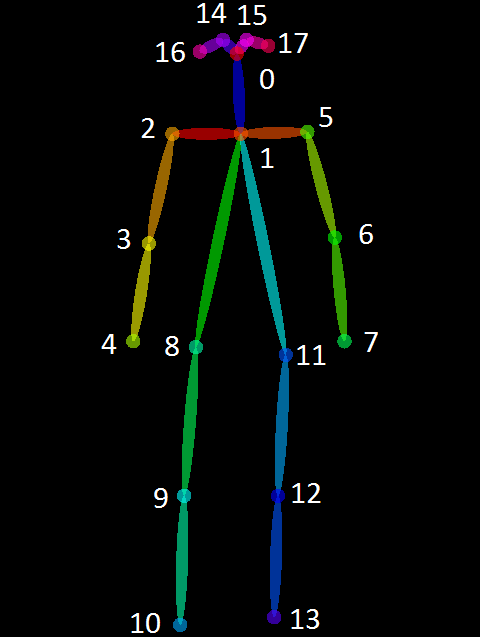
\includegraphics[width=0.4\textwidth]{./images/keypoints_pose_18.png}
	\captionsource{Numbering of the 18 keypoint of the COCO pose format from \textit{OpenPose}. \newline}{\cite{openpose}}
	\label{fig:coco}
\end{figure}
The pose output format (COCO) was used consisting of 18 keypoints as shown in figure \ref{fig:coco}. In addition to the keypoints coordinates the output also includes so called confidence scores per keypoint in the range $[0,1]$ to assess the accuracy.

\subsubsection{Algortihm}
This section is intended to give you a rough understanding of their algorithm as described in their paper \cite{openpose_paper}. Common approaches estimate the poses per person but \textit{OpenPose} follows the bottom-up approach in order to avoid runtime complexity proportional to the number of persons. So the algorithm predicts body part locations independent of the number of persons in the image and tries to connect the individual body parts so that the result are people. This is the reason for the so called buttom-up approach, but in contrast to other methods such as \textit{DeepCut}\cite{deepcut} the final analysis to map the body parts together is more efficient. 
\begin{figure}[h]
	\centering
	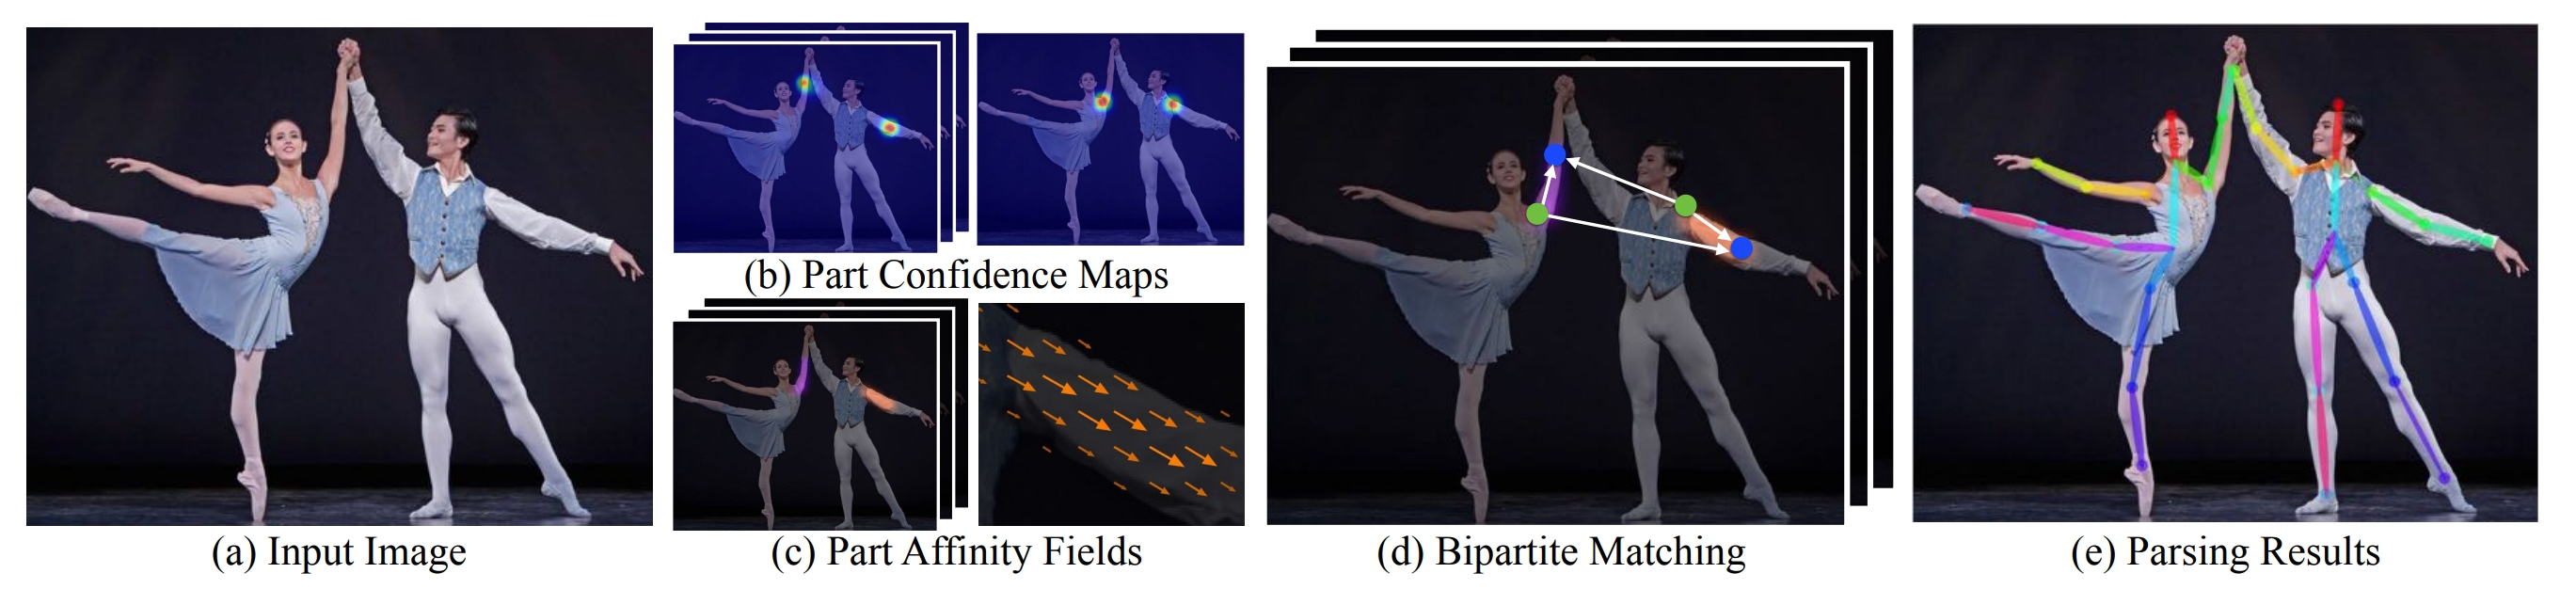
\includegraphics[width=1.\textwidth]{./images/openpose_overview.jpg}
	\captionsource{\textit{OpenPose} Pipeline Overview. The input image (a) is processed to produce the confidence maps (b) and part affinity fields (c) using a CNN. The result is formulated as a bipartite matching problem (d) in order to solve the part association (e).\newline}{\cite{openpose_paper}}
	\label{fig:openpose_overview}
\end{figure}\\
At the begin the input image is processed and analyzed using a convolutional neural network (CNN). The generated feature maps are passed into the first stage which produces a set of part affinity fields (PAFs). A 2D vector in each pixel of every PAF encodes the position and orientation of the limb which is not truly a human limb but a connection of two body parts as shown in figure \ref{fig:openpose_overview} (c). In the following stages the predictions from the previous stage and the original feature are used to refine the estimated PAFs. Afterwards the process is repeated in the same fashion for the body part location to refine the confidence maps. Each body part has its own confidence map which represents the belief for each pixel that this body part is located there as the figure \ref{fig:openpose_overview} (b) shows. So for a single person each confidence map should have one peak for the corresponding location of the body part in the image. These steps in the network differs from other approaches where both the PAFs and the body part locations are refined together but the refinement of the confidence map shows no effect on the PAFs refinement and therefore they are separated which leads to performance improvements and better accuracy. The resulting confidence map for each body part of the network is a collection of all the individual confidence maps for this body part which are combined through non-maxmimum suppression in order to not averaging along the different peaks to be able to distinguish between equal body parts that are close to each other. 
\begin{figure}[h]
	\centering
	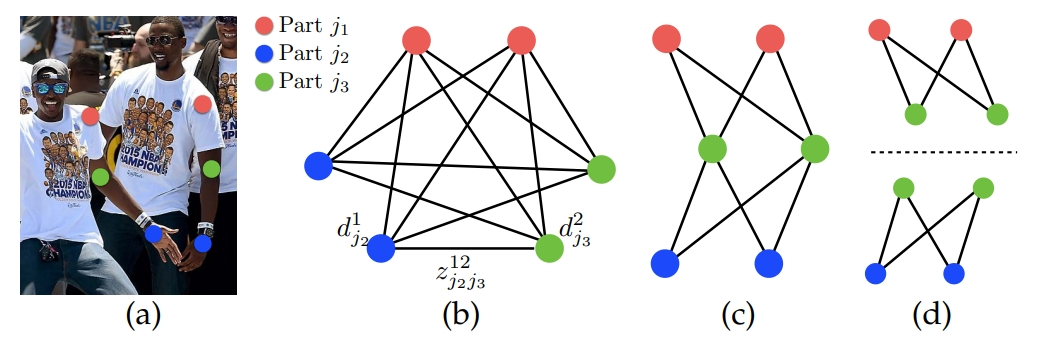
\includegraphics[width=0.8\textwidth]{./images/part_association.jpg}
	\captionsource{\textit{OpenPose's} Part Association formulated as a matching problem with the use of part affinity fields. (a) shows the detected body parts which are then connected in a complete graph (b). The first relaxation reduces the graph to spanning tree skeletons (c) and the second relaxation decompose the graph into bipartit matching subproblems (d).\newline}{\cite{openpose_paper}}
	\label{fig:openpose_mapping}
\end{figure}\\
Given the detected body parts derived from the confidence map for an unknown number of people it is now necessary to map them together to full body poses. For this purpose a confidence score for each pair of the detected body part pairs (candidate limbs) is computed using the line integral on the PAF along the connection between these two parts. Remember the PAFs preserve location and orientation that contribute the additional information needed for this step. So figure \ref{fig:openpose_mapping} (b) shows how each node represents a body part where the color corresponds to the type of body part and the edges expresses these so called candidate limbs weighted by the confidence score. So the part association problem is reformulated as a matching problem which is known to be NP-Hard. But in order to solve the matching problem efficient two relaxations are described. The first relaxation reduces the number of edges to obtain spanning tree skeletons as presented in figure \ref{fig:openpose_mapping} (c), while the second relaxation further decompose the graph into bipartit matching subproblems (d). The matching of these subproblems of adjacent tree nodes can then be determined efficiently and independently. 


\subsection{Depth Map Estimation}
% TODO: eventuell noch depth map estimation erklären wie es gelöst wurde

\section{Filterpy}\label{sec:filterpy}
% some information about the library and the book
FilterPy is a Python library that implements a number of Bayesian filter like for example the Extended Kalman Filter. The author of the library also wrote a book named \textit{Kalman and Bayesian Filter in Python} \cite{filterpybook}. Because the free book was written using Ipython Notebook, it offers the perfect interactive guide to deal with bayesian filter. It starts with some simple filters up to the Kalman filter. It describes the implementation of the library with many examples and explains the mathematical background to understand why it works. For more information visit the the github page \cite{filterpygithub}. 